\documentclass[slidestop, compress, mathserif, blackandwhite, utf8, serif, slidescentered]{beamer}

\usepackage{cmap} % для кодировки шрифтов в pdf
\usepackage[T2A]{fontenc}
\usepackage[utf8]{inputenc}
\usepackage[russian]{babel}
\usepackage{pscyr}
\renewcommand{\rmdefault}{ftm}
\usepackage{float}
\usepackage{makecell}
\usepackage{multirow} % улучшенное форматирование таблиц
\usepackage{ulem} % подчеркивания
\usepackage{enumerate}
\usepackage{amssymb,amsfonts,amsmath,amsthm} % математические дополнения от АМС
\usepackage{graphicx} % для вставки картинок

\usepackage[tableposition=top]{caption}
\usepackage{subcaption}
%\usepackage{subfig}
\DeclareCaptionFont{small}{\small}
\DeclareCaptionLabelFormat{gostfigure}{\small Рисунок #2}
\DeclareCaptionLabelFormat{gosttable}{Таблица #2}
\DeclareCaptionLabelSeparator{gost}{~---~}
\captionsetup{labelsep=gost,font=small}
\captionsetup[figure]{labelformat=gostfigure}
\captionsetup[table]{labelformat=gosttable}
\renewcommand{\thesubfigure}{\asbuk{subfigure}}
\renewcommand{\thefigure}{\arabic{figure}}


\usetheme{Antibes}
\title{Исследование алгоритмов\\ распознавания речи}
\author{Ряховский Александр Александрович}
\institute{Национальный Исследовательский Университет\\ <<Белгородский Государственный Университет>>}
\date{\\ 2012}

\begin{document}
%\maketitle
\section{Введение}
\begin{frame}[plain]
	\frametitle{Актуальность работы}
	В настоящее время, с развитием компьютерных технологий, использование систем автоматического распознавания речи в качестве интерфейса приобретает все большую популярность. Cоздание таких систем является нетривиальной задачей.

	Успешное решение данной проблемы позволит осуществить частичную замену интеллектуальной деятельности человека действием автоматов.
\end{frame}
\begin{frame}[plain]
	\frametitle{Цели и задачи}
	Целью работы является реализация и исследование алгоритма распознавания речи.\\~\\

	Для достижения поставленной цели требуется решить следующие задачи:
	\begin{enumerate}[1)]
		\item Провести анализ моделей речевого сигнала;
		\item Изучить подходы к решению задачи распознавания устной речи;
		\item Реализовать алгоритм получения описания речевого сигнала и решающую функцию;
		\item Исследовать реализованный алгоритм.
	\end{enumerate}
\end{frame}

\section{Мел-частотные кепстральные коэффициенты (MFCC)}
\begin{frame}[shrink,plain]
	\frametitle{Описание речевых сигналов}
	При распознавании речевых сигналов, как правило, оперируют не с исходным речевым сигналом, получаемым на выходе микрофона, а с так называемым описанием речевого сигнала.\\~\\

	Так, исходный речевой сигнал, который характеризуется объемом 256 кбит/с, как правило, описывается существенно меньшим объемом информации --- от 9600 до 600 и менее бит/с\\~\\

	Элементы описания могут содержать компоненты, описываемые разнородными физическими величинами. Например, наряду с компонентами, представляющими форму амплитудного спектра речи или передаточную характеристику речевого тракта, могут быть компоненты, характеризующие интенсивность элемента, способ eгo образования, относительную частоту основного тона и т. п.

\end{frame}

\begin{frame}[shrink,plain]
	\frametitle{Кепстральный анализ}
	Основой кепстрального анализа речевых сигналов является предположение, что речевой сигнал трактуется как сигнал на выходе линейной системы с медленно изменяющимися параметрами.
	\begin{figure}[h]	
	\centering
	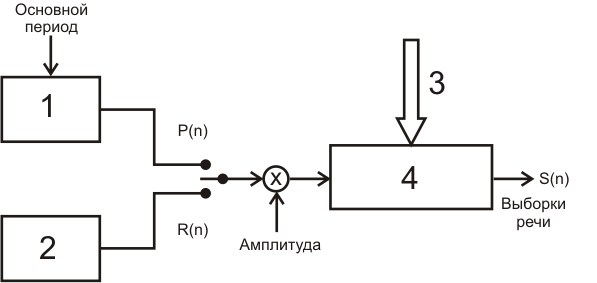
\includegraphics[width=.7\textwidth]{../speech_filt.png}			
	\caption{\centering{Модель речевого аппарата в виде линейной системы -- \linebreak 1) Генератор импульсной последовательности; 2) Генератор случайных чисел; 3) Коэффициенты цифрового фильтра (параметры голосового тракта); 4) Нестационарный цифровой фильтр.}}
	
	\label{speech_filt}
	\end{figure}
\end{frame}

\begin{frame}[shrink,plain]
	\frametitle{Кепстральный анализ}
	Рассматриваемые фильтры имеют постоянные характеристики на временном интервале порядка 10-15 мс. Поэтому на каждом интервале фильтр можно характеризовать импульсной или частотной характеристикой или набором коэффициентов, если импульсная характеристика фильтра бесконечна. Такая модель позволяет применить для анализа речевых сигналов гомоморфную развертку.

	Выходной сигнал определяется сверткой:
	\begin{equation}
		s_{\text{вых}}(t)=s_{\text{вх}}(t)\otimes h(t);
	\end{equation}
	
	\begin{equation}
		S_{\text{вых}}(\omega)=S_{\text{вх}}(\omega)H(\omega)	
	\end{equation}
	   
	\begin{equation}
		ln[S^2_{\text{вых}}(\omega)]=ln[S^{2}_{\text{вх}}(\omega)]+ln[H^{2}(\omega)].
		\label{eq:unconv1}
	\end{equation}

\end{frame}

\begin{frame}[plain]
	\frametitle{Кепстральный анализ}
	Применив к (\ref{eq:unconv1}) обратное преобразование Фурье, можно получить выражение вида:

	\begin{equation}
		C(q)=C_{s}(q)+C_{h}(q)
	\end{equation}

	из которого методами линейной фильтрации может быть возможно выделить некоторые характеристики $s_{\text{вх}}(t)$ и $h(t)$.

	Также $C(q)$ может быть записано в виде:
	\begin{equation}
		 C(q)={\frac{1}{2\pi}}\int\limits_{-\infty}^{\infty} \ln [S(\omega)]^2 e^{i\omega q}\, d\omega .
	\end{equation}
	Данное преобразование получило название <<кепстр>>.
\end{frame}

\begin{frame}[plain]
	\frametitle{Кепстральный анализ}
	Так как рассматриваемые в данной работе системы распознавания речи работают с дискретным представлением речевого сигнала, целесообразно привести запись кепстра в дискретной форме:
	\begin{equation}
		C(n)=\frac{1}{N}\sum_{k=0}^{N-1}{\ln|{X(k)}|^2e^{i\frac{2\pi}{N}kn}}, \; 0\leq n\leq N-1.
	\end{equation}

\end{frame}	

\begin{frame}[plain]
	\frametitle{Мел-частотные кепстральные коэффициенты}
	Представление спектра сигнала в виде мел-частотных коэффициентов может успешно применяться в распознавании речи. Значения коэффициентов в шкале мел могут быть получены, анализируя значения коэффициентов в шкале Герц с последующим переходом при использовании выражения:
	\begin{equation}
		B(f)=1125\ln(1+f/700)
		\label{eq:mel}
	\end{equation}
	где  $f$ --- значение частоты в Герцах;\\
	$B(f)$ --- значение частоты в мел, соответствующее частоте в Герцах $f$.


\end{frame}

\begin{frame}[plain]
	\frametitle{Мел-частотные кепстральные коэффициенты}
	
	\begin{figure}[h]
		\centering
		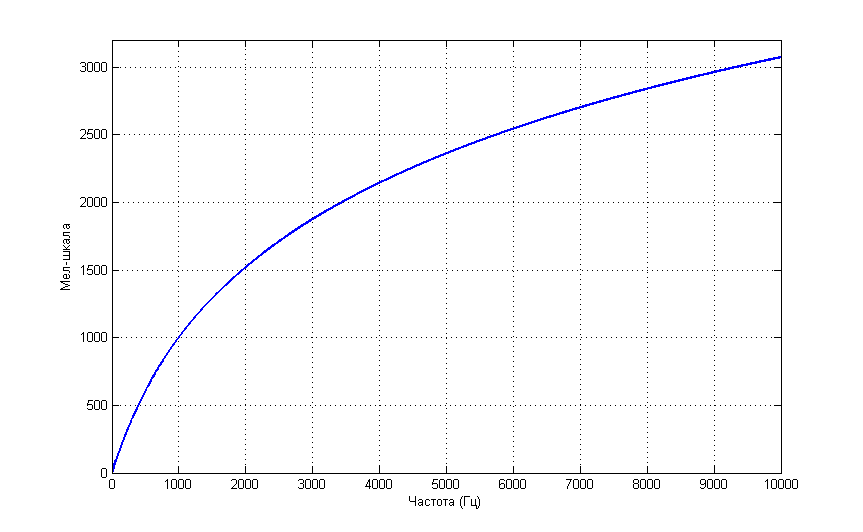
\includegraphics[width=.8\textwidth]{mel-scale.png}
		\caption{Зависимость высоты звука в мелах от частоты}
		\label{mfcc_number}
	\end{figure}

\end{frame}

\begin{frame}[plain]
	\frametitle{Мел-частотные кепстральные коэффициенты}
	Для оценки значений мел-частотных кепстральных коэффициентов на первом этапе необходимо оценить значения трансформанты Фурье анализируемого фрагмента сигнала вида:
	\begin{equation}
		X_{k} =\sum_{n=0}^{N-1}x_{n}e^{\frac{-2\pi i}{N} kn},  \;\; 0\le k<N_f,
	\end{equation}
	где  $x_n$ --- анализируемый отрезок сигнала, длительностью $N$ отсчетов; $N_f$ --- количество точек Фурье.
\end{frame}

\begin{frame}[plain]
	\frametitle{Мел-частотные кепстральные коэффициенты}
	При оценке логарифмов значений трансформант Фурье предлагается использовать треугольную оконную функцию вида:
	\begin{equation}
		H_{m}=
		\begin{cases}
			0,&k<f_{m-1}\\ 
			\frac{(k-f_{m-1})}{(f_{m}-f_{m-1})},&f_{m-1} \leq k < f_{m}\\ 
			\frac{(f_{m+1}-k)}{(f_{m+1}-f[m])},&f_{m} \leq k \leq f_{m+1}\\ 
			0,&k > f_{m+1}
		\end{cases}
		\label{eq:window}
	\end{equation}
	где $f_m$ – граничная частота m-го окна.

\end{frame}

\begin{frame}[plain]
	\frametitle{Мел-частотные кепстральные коэффициенты}

	\begin{figure}[h]
		\centering
		\begin{subfigure}{0.49\textwidth}
		\centering
		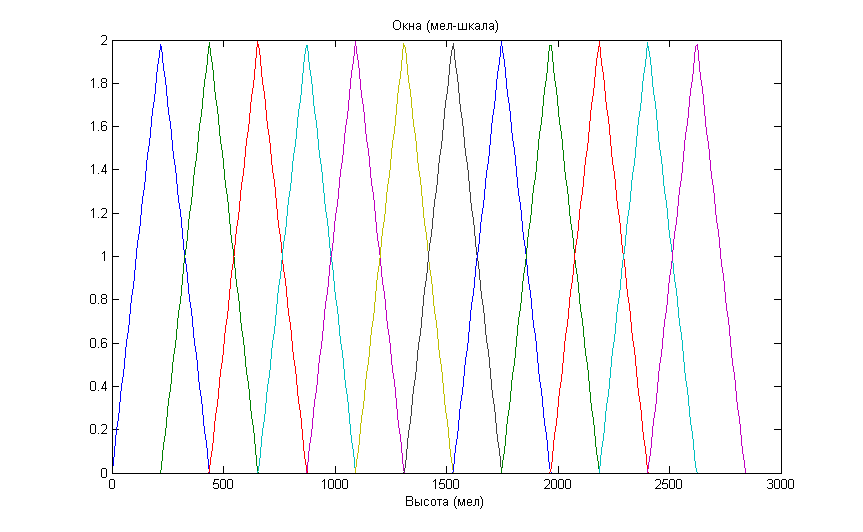
\includegraphics[width=.99\textwidth]{graph-3.png}
		\caption{}		
		\end{subfigure}
		\begin{subfigure}{0.49\textwidth}
		\centering
		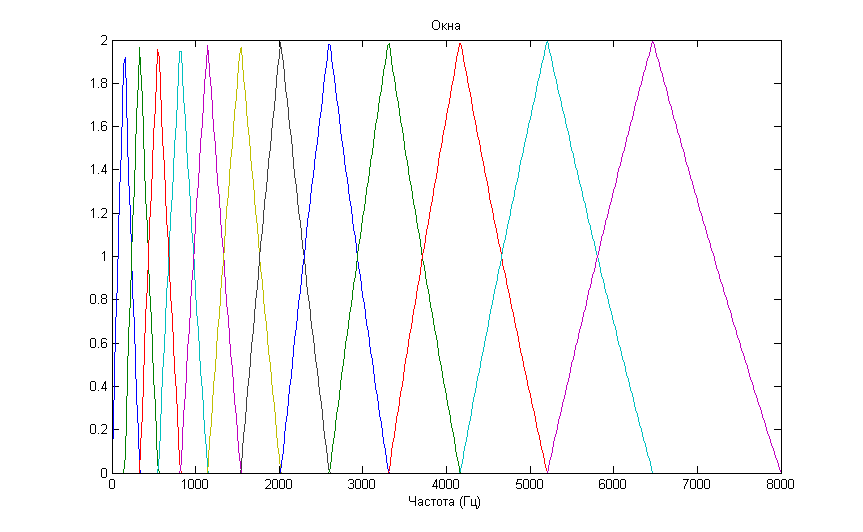
\includegraphics[width=.99\textwidth]{graph-4.png}
		\caption{}			
		\end{subfigure}
		\caption{\parbox[t]{.59\textwidth}{Графики оконных функций для 12 окон: \\ а) в шкале мел; \\ б) в шкале Гц}}
		\label{mel_scale}
	\end{figure}


\end{frame}




 \begin{frame}[plain]
 	\frametitle{Мел-частотные кепстральные коэффициенты}
	Для оценки кепстральных коэффициентов необходимо оценить значения логарифмов результата дискретного преобразования Фурье:
	\begin{equation}
		S_m=\ln(\sum_{k=0}^{N-1}|X_k|^2 H_{m,k}), \; \; 0\leq m \le M,
		\label{eq:cepstr}
	\end{equation}
	где $X_k$ -- значения трансформанты Фурье;\\
	$M$ -- число треугольных окон, равномерно расположенных в шкале мел;\\
	$H_{m,k}$ -- значения оконной функции вида (\ref{eq:window}).

 \end{frame}

 \begin{frame}[plain]
 	\frametitle{Мел-частотные кепстральные коэффициенты}
	Затем к полученным результатам применяются дискретное косинусное преобразование:
	\begin{equation}
		c_n=\sum_{m=0}^{M-1}S_m cos(\pi n(m+\frac{1}{2})/M), \; \; 0\leq n \le M,
	\end{equation}
	где  $M$ – количество треугольных окон, равномерно распределенных в шкале мел;\\
	$S_m$ – значение результата логарифмирования вида (\ref{eq:cepstr}).

 \end{frame}

 \begin{frame}[plain]
 	\frametitle{Мел-частотные кепстральные коэффициенты}
 	\hfill
	\begin{figure}[h]
	\centering
	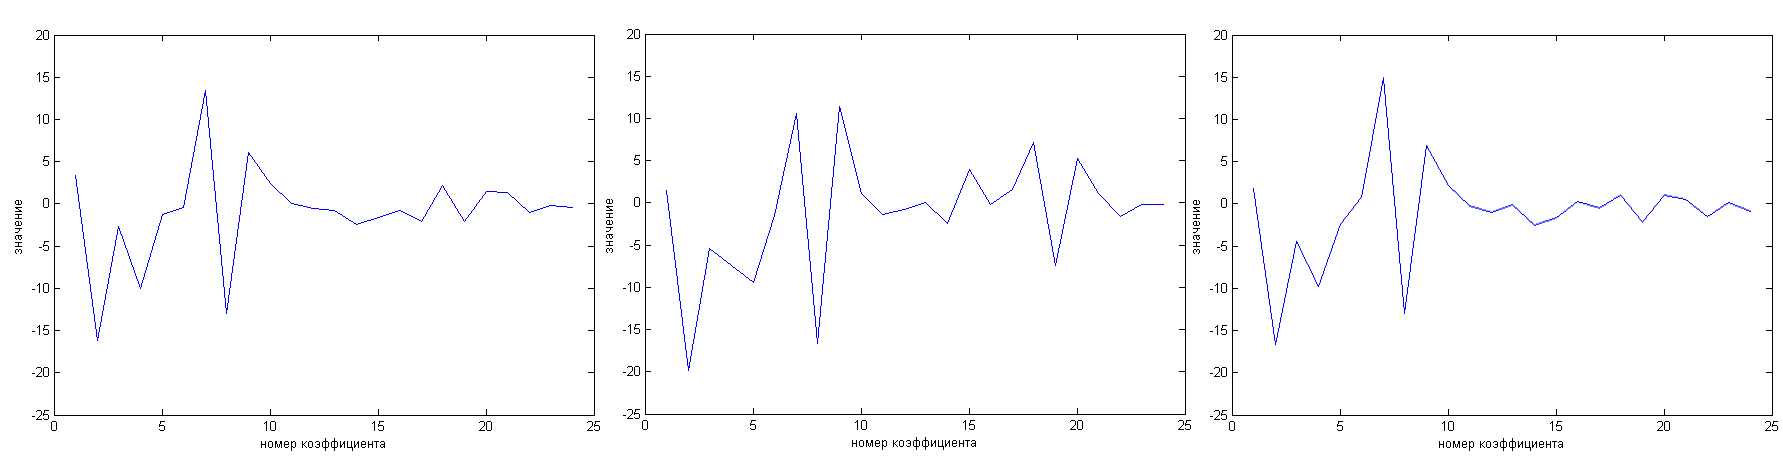
\includegraphics[width=\textwidth]{a_mfcc_horz.png}
	\caption{\centering{Наборы мел-кепстральных коэффициентов для трех реализаций звука <<а>>}}
	\label{a_mfcc}
\end{figure}

 \end{frame}

 \begin{frame}[plain]
 	\frametitle{Мел-частотные кепстральные коэффициенты}
 	\hfill
	\begin{figure}[h]
	\centering
	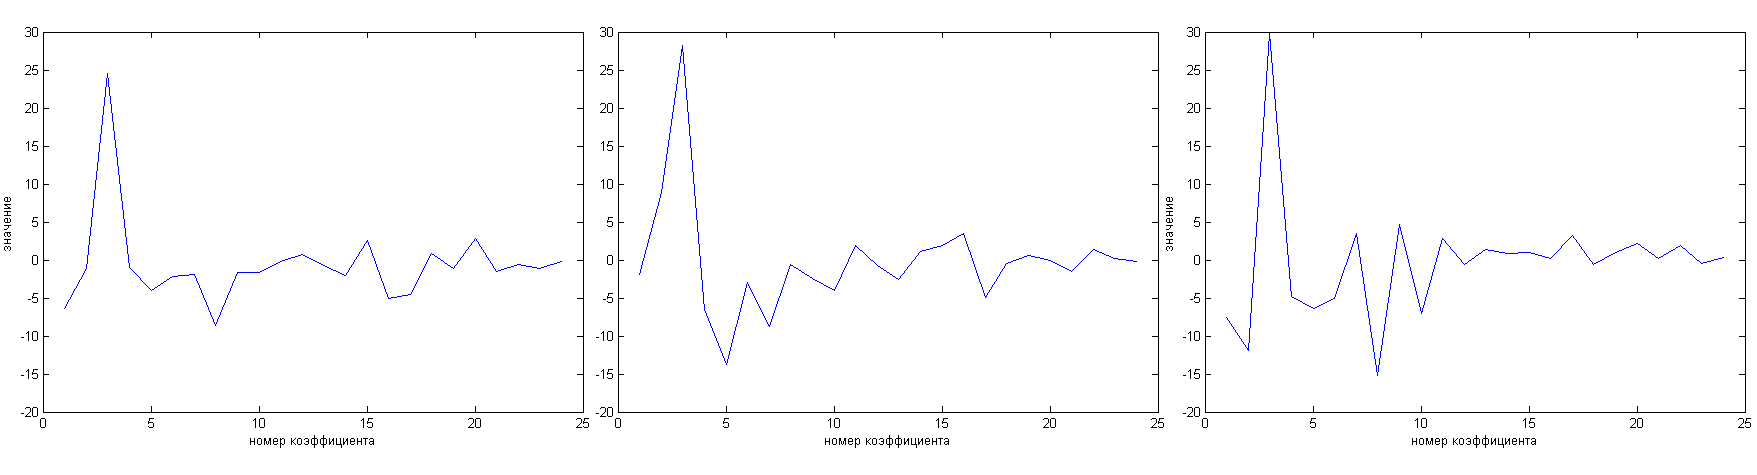
\includegraphics[width=\textwidth]{i_mfcc_horz.png}
	\caption{\centering{Наборы мел-кепстральных коэффициентов для трех реализаций звука <<и>>}}
	\label{a_mfcc}
	\end{figure}

 \end{frame}

\begin{frame}[plain]
 	\frametitle{Мел-частотные кепстральные коэффициенты}
	В проведенных экспериментах анализировались отрезки сигнала длиной в 256 отсчетов (16 мс при используемой частоте дискретизации 16 кГц) с перекрытием в 128 отсчетов, с целью обеспечения относительной стационарности анализируемого речевого отрезка. Количество точек Фурье устанавливалось равным длине отрезка.\\~\\

	Количество используемых коэффициентов установлено равным 24 на основании рекомендаций, приведенных в литературе. Также было исследовано влияние количества используемых коэффициентов на точность распознавания речевых сигналов. В эксперименте рассчитывались все 24 коэффициента, а затем для описания сигнала в алгоритме распознавания использовались $N_k$ коэффициентов.

\end{frame}

\begin{frame}[plain]
	\frametitle{Мел-частотные кепстральные коэффициенты}
	\begin{figure}[h]
		\centering
		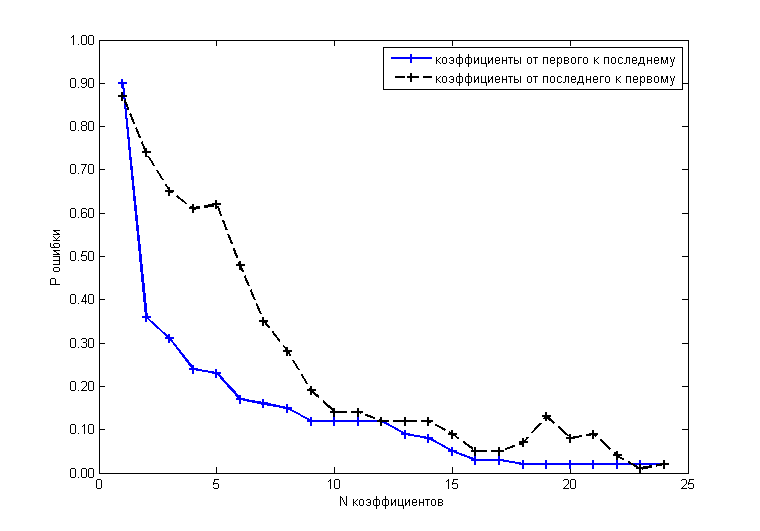
\includegraphics[width=.8\textwidth]{../decrease_legend.png}
		\caption{\centering{Зависимость вероятности ошибки распознавания от количества используемых коэффициентов}}
		\label{a_mfcc}
	\end{figure}

\end{frame}

\section{Алгоритм динамического трансформирования времени}
\begin{frame}[plain]
	\frametitle{Динамическое программирование}
	\textbf{Динамическое программирование} — способ решения сложных задач путём разбиения их на более простые подзадачи.\\~\\

	В применении к задачам распознавания речи методы динамического программирования используются для определения степени схожести речевых сигналов. Как правило, подобное сравнение входного сигнала с имеющимся образцом имеет место в системах распознавания, работающих с ограниченным словарем (до 50 слов), но может также применяться на отдельных этапах принятия решений в составе комплексных систем.

\end{frame}

\begin{frame}[plain]
	\frametitle{Алгоритм динамического трансформирования времени}
	Одно и то же сочетание звуков может иметь различную длительность, что создает проблему для системы распознавания. Использование алгоритма динамического трансформирования времени позволяет избежать этой проблемы.\\~\\

	Алгоритм динамического трансформирования времени (англ. Dynamic Time Warp или DTW) вычисляет оптимальную последовательность трансформации (деформации) времени между двумя временными рядами. Алгоритм вычисляет оба значения деформации между двумя рядами и расстояние между ними.
\end{frame}

\begin{frame}[plain]
	\frametitle{Алгоритм динамического трансформирования времени}
	Предположим, что есть две числовые последовательности $A= a_{1}, a_{2}, \dots, a_{I}$ и $B=b_{1}, b_{2}, \dots, b_{J}$. Длина двух последовательностей может быть различной.

	Временные различия между A и B могут быть описаны с помощью некоторой последовательности $c=(i,j)$:
	\begin{equation}
		F=c(1),c(2)\dots,c(k),\dots,c(K)
		\label{eq:F}
	\end{equation}
	где $c(k)=(i(k),j(k))$.
	Данная последовательность представляет собой функцию, которая позволяет отобразить временную ось A на временной оси B. Назовем ее функцией деформации.
\end{frame}

\begin{frame}[plain]
	\frametitle{Алгоритм динамического трансформирования времени}
	\begin{figure}[h]	
	\centering
	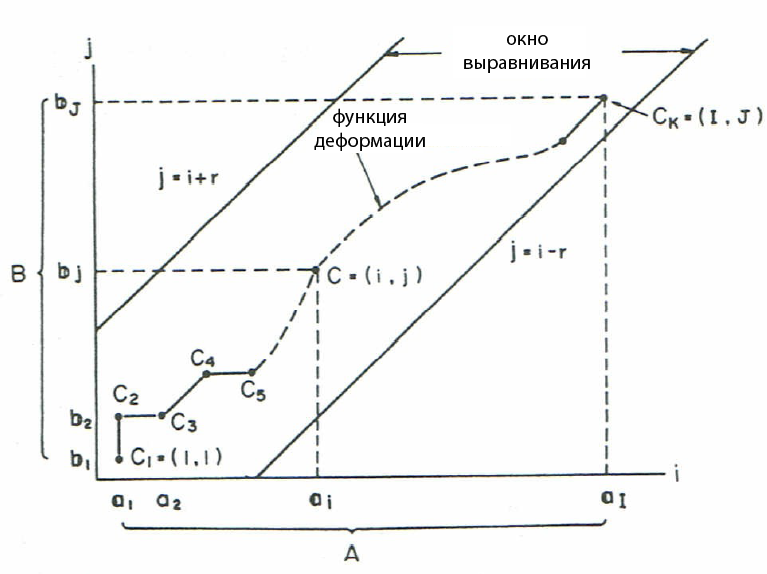
\includegraphics[width=.6\textwidth]{../sakoe1.png}			
	\caption{Функция деформации и окно выравнивания}
	\label{sakoe1}
	\end{figure}
\end{frame}

\begin{frame}[plain]
	\frametitle{Алгоритм динамического трансформирования времени}
	Алгоритм начинается с расчета локальных расстояний между элементами двух последовательностей. 
	В рамках данной работы при реализации алгоритма динамического трансформирования используются коэффициенты корреляции Пирсона, рассчитанные для кепстральных коэффициентов отрезков сигнала:
	\begin{equation}
		d(i,j)=1-\frac{\sum_{k-1}^{M}c1_{i,k}\cdot c2_{i,k}}{\sqrt{\sum_{k-1}^{M}c1_{i,k}^2 \cdot c2_{i,k}^2}}, \; \; 1 \leq i \leq I, \; 1 \leq j \leq J,
		\label{eq:pirson}
	\end{equation}
	где с1, с2 – кепстральные коэффициенты соответственно первого и второго сигнала;\\
	I, J – длительности соответственно первого и второго сигнала;\\
	М – количество кепстральных коэффициентов, используемых для анализа.
\end{frame}

\begin{frame}[plain]
	\frametitle{Алгоритм динамического трансформирования времени}
	В результате получаем матрицу расстояний, имеющую I строк и J столбцов общих членов:
	\begin{equation}
		d(c)=d(i,j)
	\end{equation}
	 Минимальное остаточное расстояние между A и B, которое остается после устранения временных различий, может служить мерой различия речевых последовательностей A и B
	\begin{equation}
		Dist(A,B)=min_F\left[\frac{\sum_{k=1}^{K}{d(c(k))\cdot w(k)}}{\sum_{k=1}^{K}{w(k)}}\right]
		\label{eq:dist}
	\end{equation}
	где $w(k)$ - неотрицательный весовой коэффициент.
\end{frame}

\begin{frame}[plain]
	\frametitle{Алгоритм динамического трансформирования времени}
	Существует три условия, налагаемых на DTW алгоритм для обеспечения быстрой конвергенции:

	\begin{enumerate}[1)]
	\item Монотонность – путь никогда не возвращается, то есть: оба индекса, $i$ и $j$, которые используются в последовательности, никогда не уменьшаются. 

	\item Непрерывность – последовательность продвигается постепенно: за один шаг индексы $i$ и $j$, увеличиваются не более чем на 1.

	\item Предельность – последовательность начинается в $(1,1)$ и заканчивается в $(I,J)$.
	\end{enumerate}
	Вычислительная сложность реализованного алгоритма составляет порядка $O(IJ)$, возможно, сложность может быть уменьшена оптимизацией алгоритма.
\end{frame}

\begin{frame}[plain]
	\frametitle{Блок-схема алгоритма}
	\begin{figure}[h]	
	\centering
	\begin{subfigure}{0.49\textwidth}
		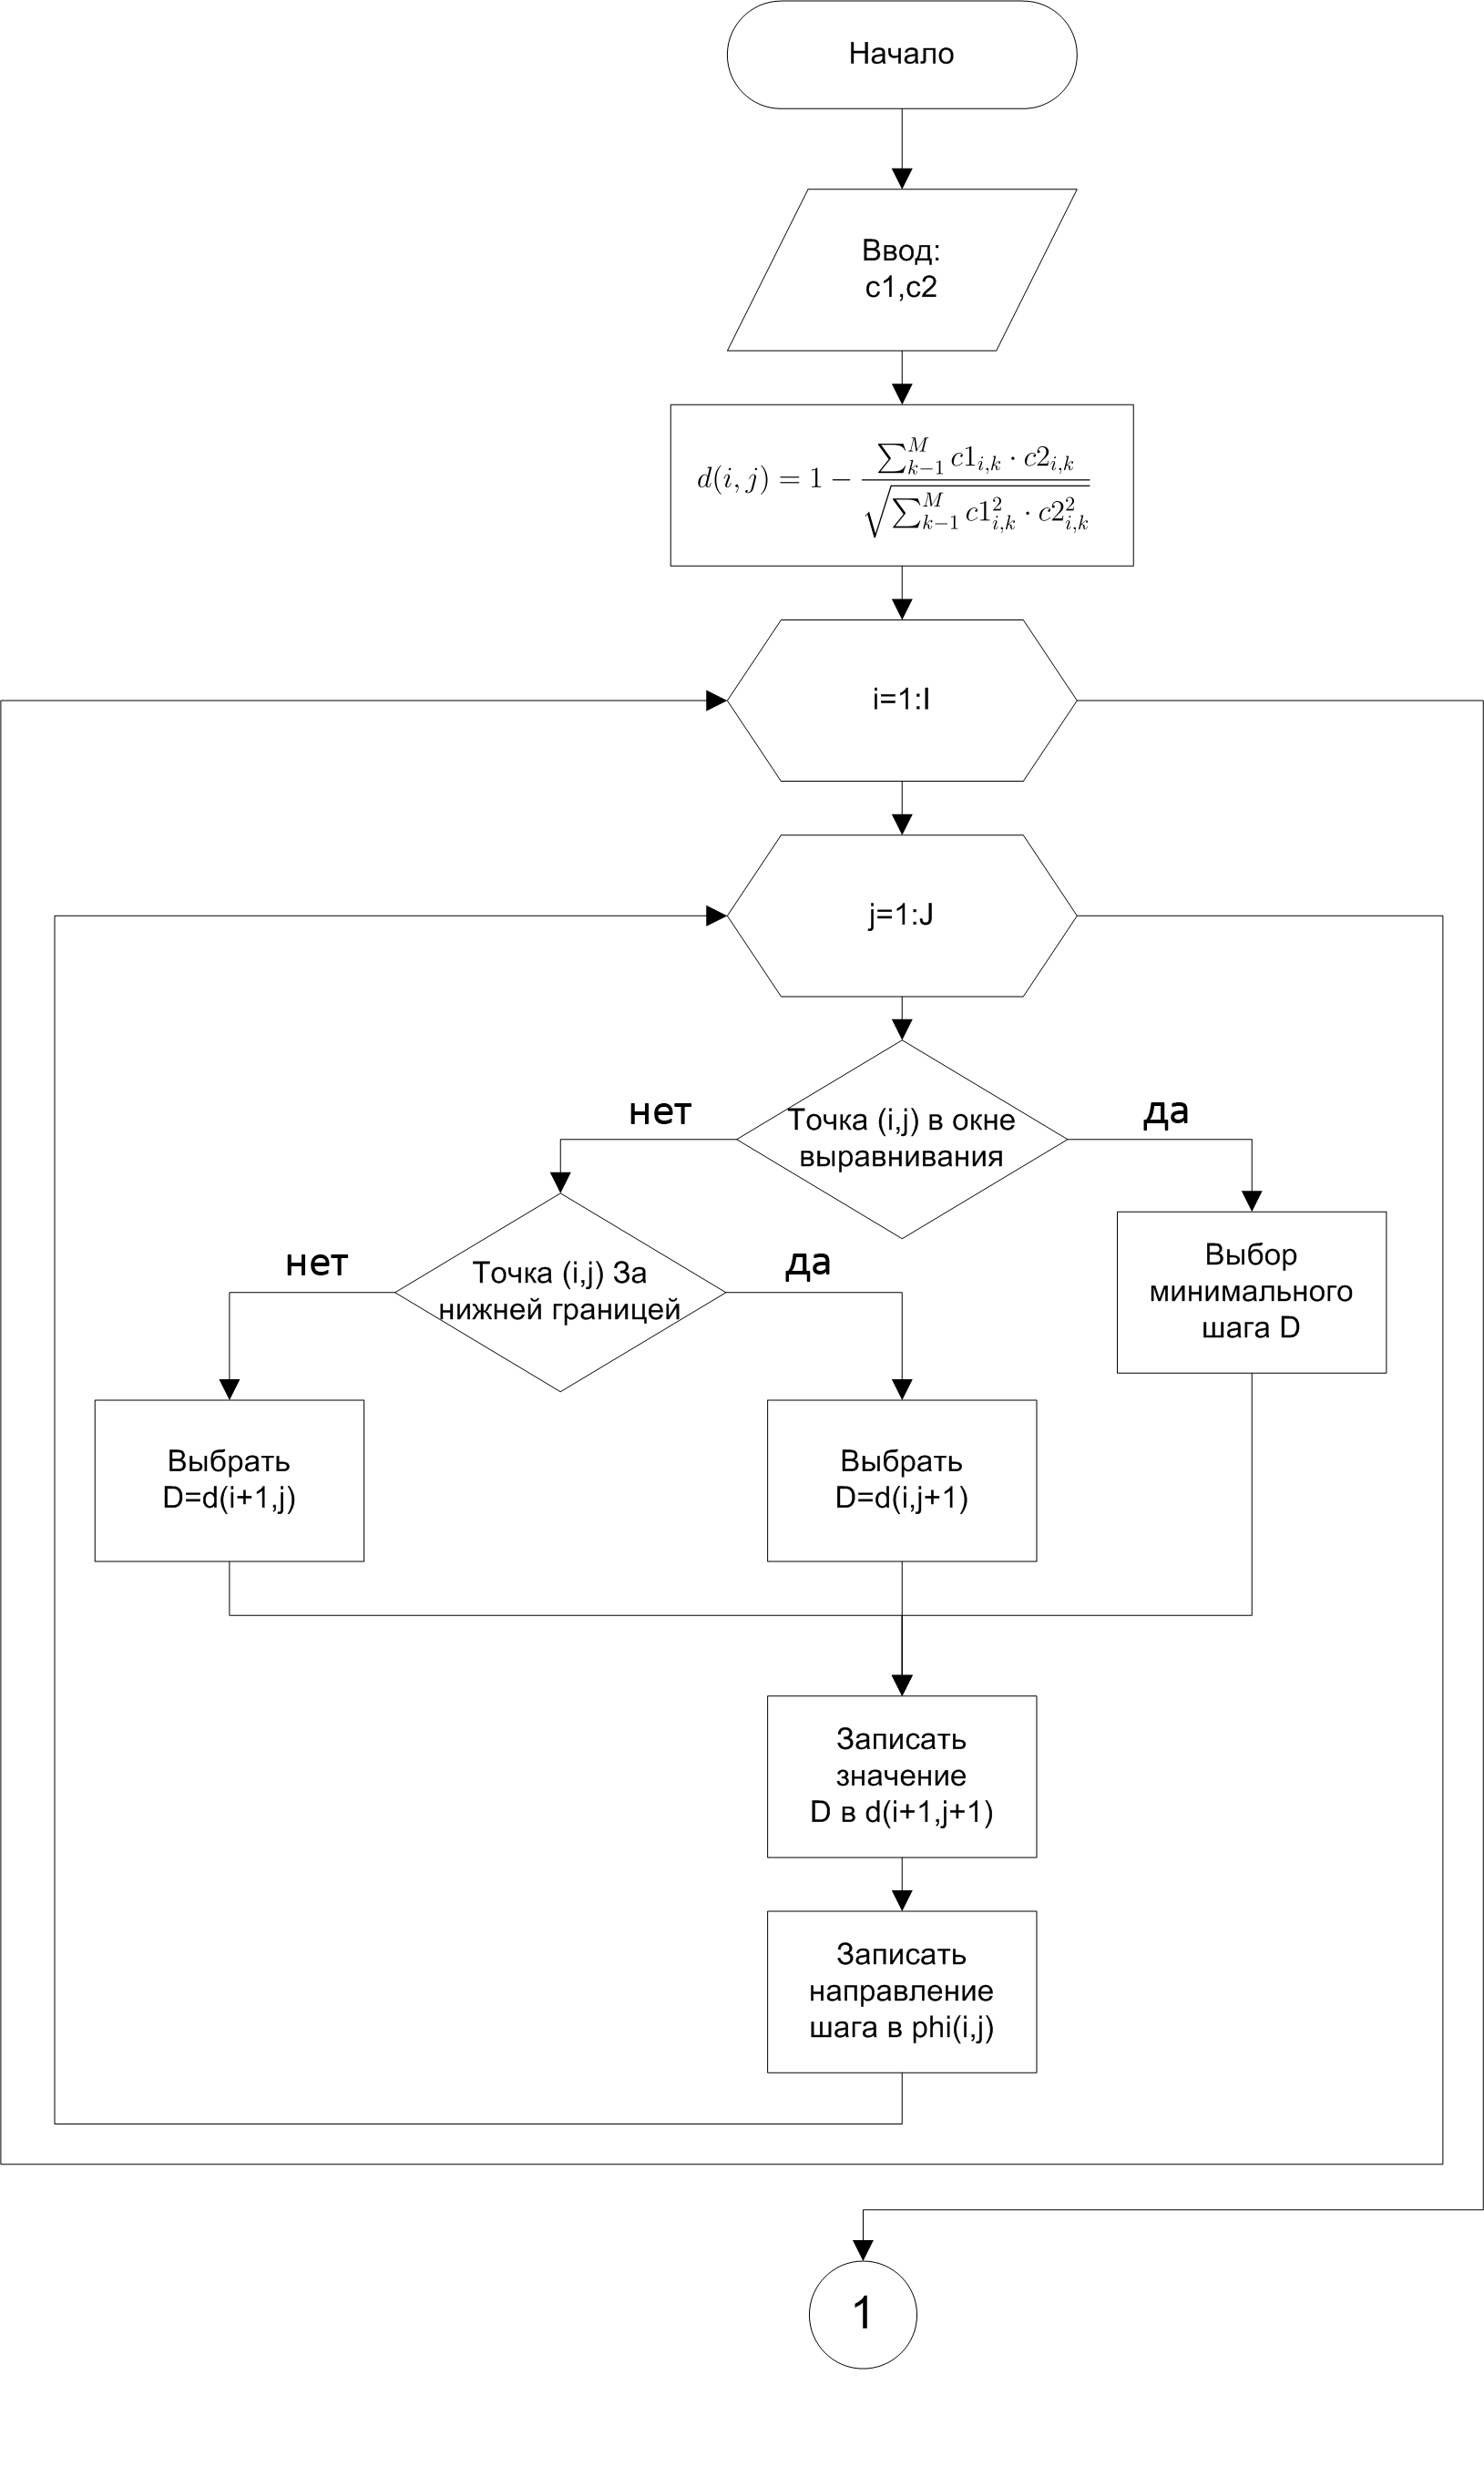
\includegraphics[width=.8\textwidth]{../block1.png}			
	\end{subfigure}
	\begin{subfigure}{0.49\textwidth}
		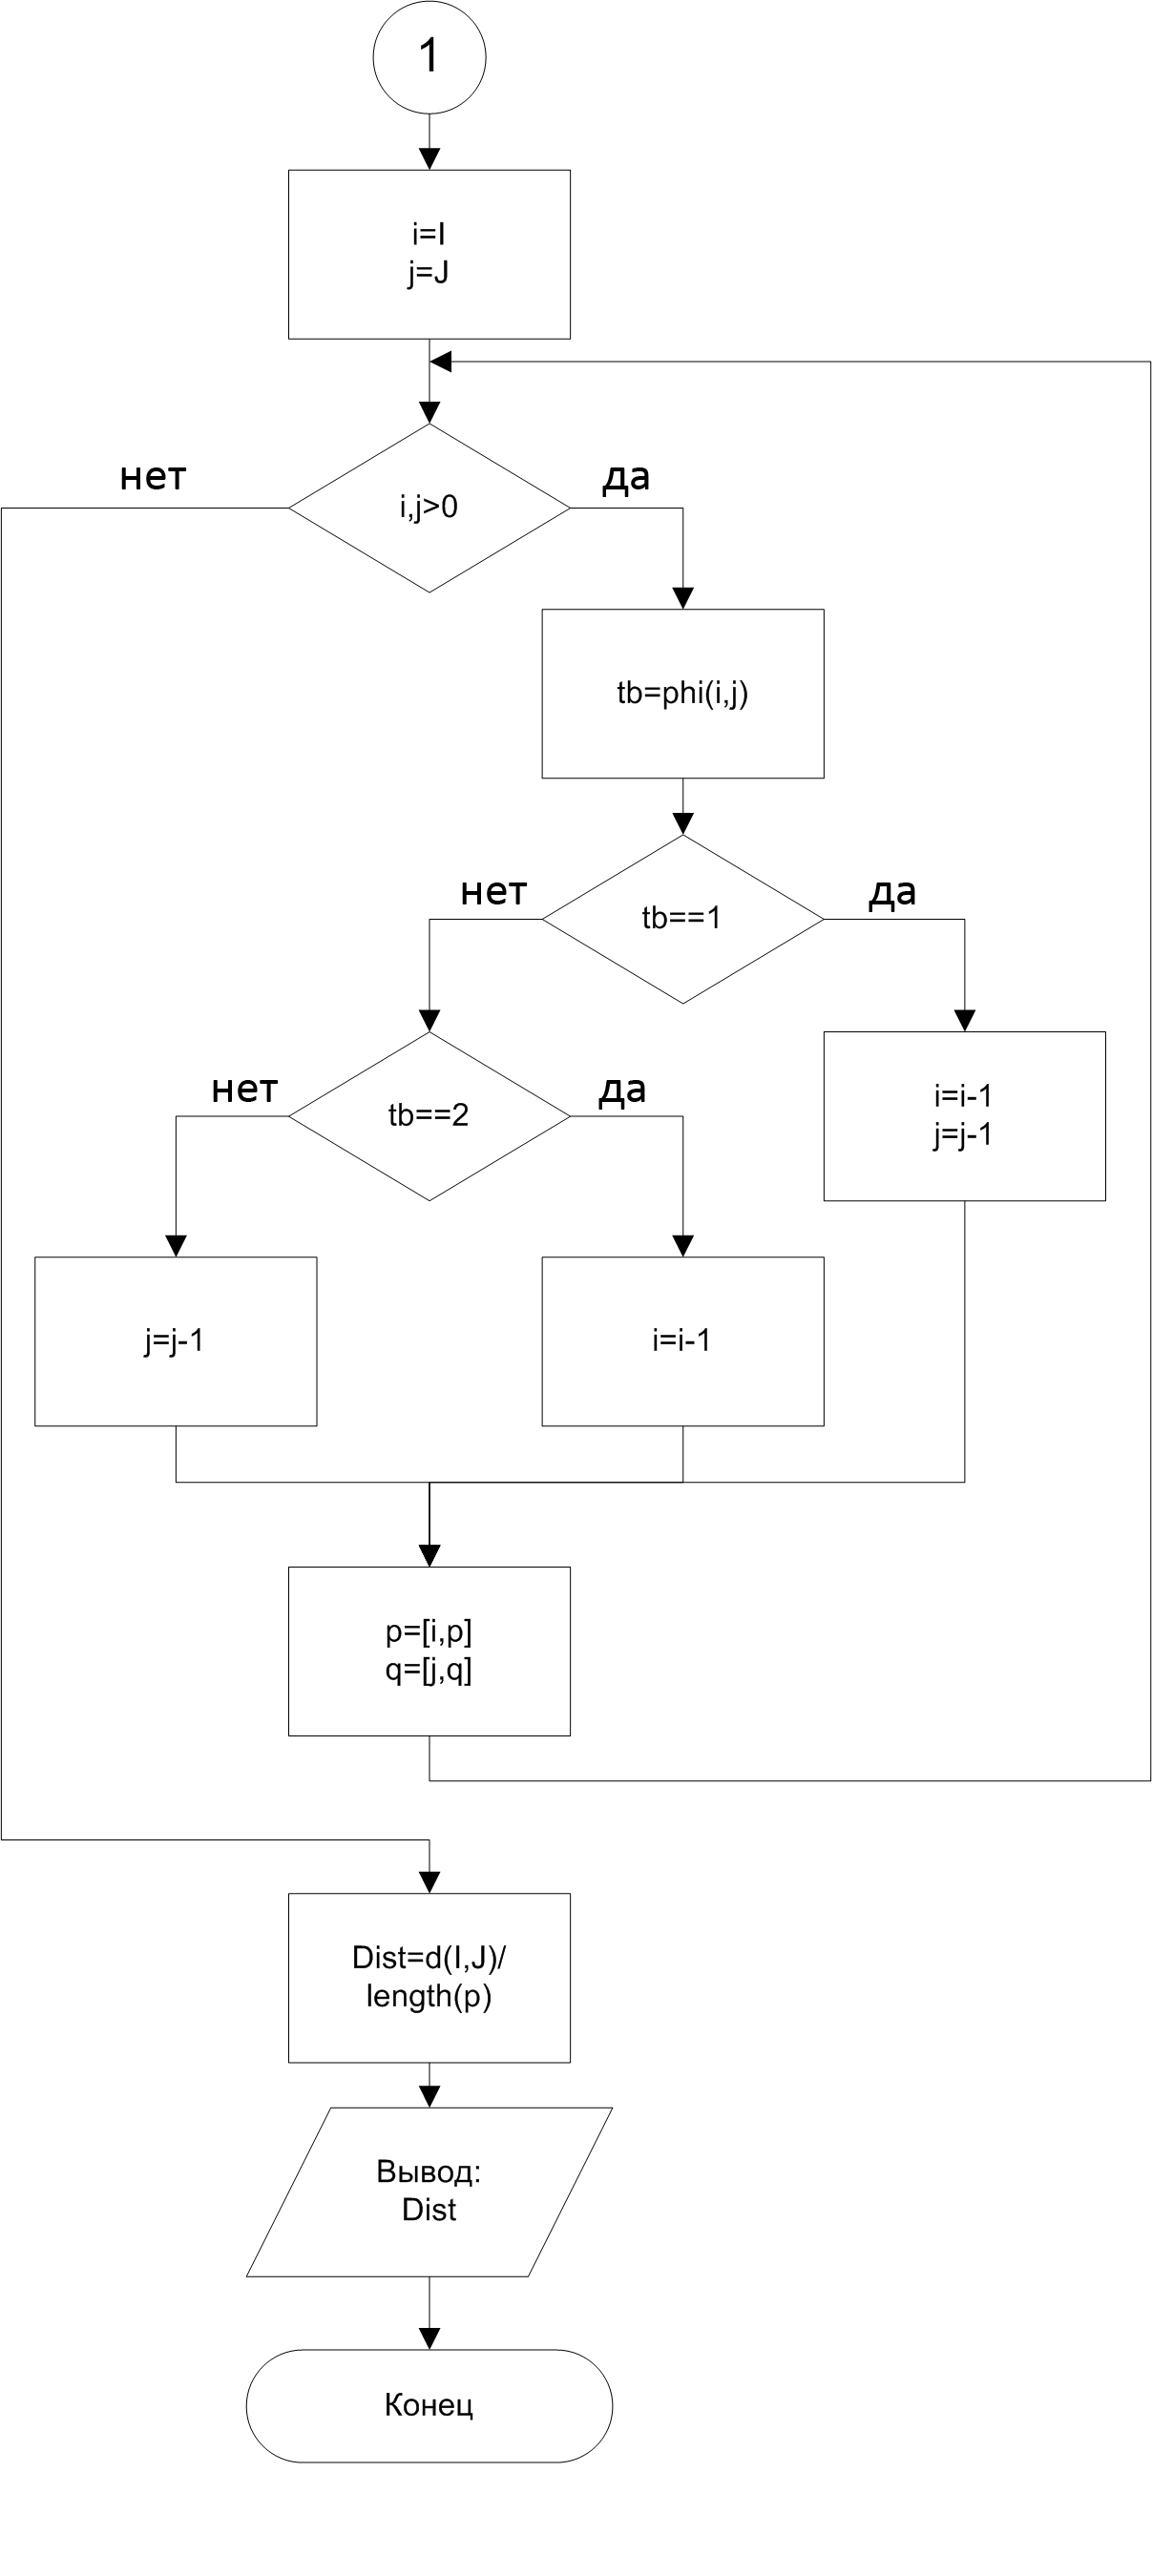
\includegraphics[width=.59\textwidth]{../block2.png}			
	\end{subfigure}

	\label{block1}
\end{figure}
\end{frame}

\begin{frame}[plain]
	\frametitle{Алгоритм динамического трансформирования времени}
	\begin{figure}[h]	
	\centering
	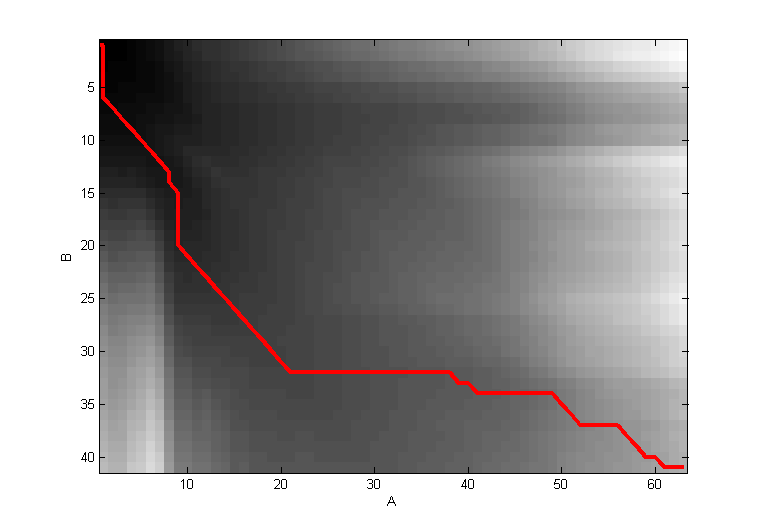
\includegraphics[width=.7\textwidth]{../d_matrix.png}			
	\caption{Функция $F$ вида (\ref{eq:F}), наложенная на матрицу $d$}
	\label{d_matrix}
	\end{figure}
\end{frame}

\begin{frame}[plain]
	\frametitle{Алгоритм динамического трансформирования времени}
	
	С помощью данного алгоритма производится сравнение анализируемого сигнала с сохраненными в памяти компьютера эталонами. В результате выбирается пара с минимальной дистанцией и делается вывод о соответствии сигнала слову из словаря.

	\begin{figure}[H]	
	\centering
	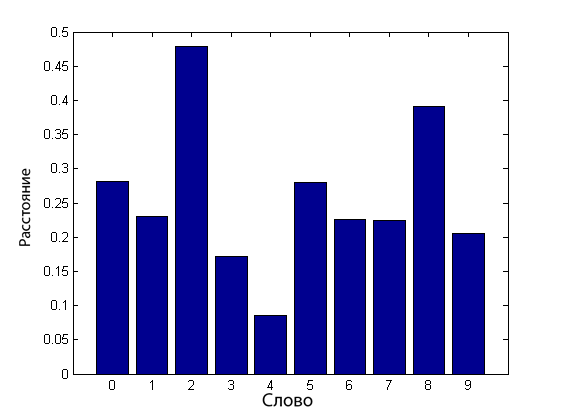
\includegraphics[width=.44\textwidth]{../dist_4.png}
	\caption{Значения меры отличий для слова «четыре»}
	\label{dist_4}
	\end{figure} 

\end{frame}

\begin{frame}[plain]
	\frametitle{Алгоритм динамического трансформирования времени}
	Для исследования данного алгоритма была составлена база эталонов из 10 слов (числительные от 0 до 9). В качестве исходного сигнала использовались записи речевого сигнала с частотой дискретизации 16 кГц и разрядностью кода 16 бит. Исследование вероятностей ошибочного принятия решения осуществлялось на основе анализа 10 повторений этих же числительных тем же диктором (100 образцов). В результате, на 100 повторений было обнаружено 2 ошибки распознавания, что позволяет говорить о достаточной степени точности выбранного алгоритма.
\end{frame}	

\begin{frame}[plain]
	\frametitle{Алгоритм динамического трансформирования времени}
	К достоинствам выбранного алгоритма можно отнести достаточно высокую точность распонавания при работе с небольшим словарем, относительно небольшую сложность реализации и устойчивость к различиям в скорости произношения анализируемых слов. Однако, данный алгоритм обладает и рядом недостатков, таких как ограниченность размера используемого словаря, чувствительность к точности выделения слова из речевого потока и влиянию шумов.
\end{frame}	

\begin{frame}[plain]
	\frametitle{Алгоритм динамического трансформирования времени}
	\begin{figure}[h]
		\begin{subfigure}{0.32\textwidth}	
			\centering
			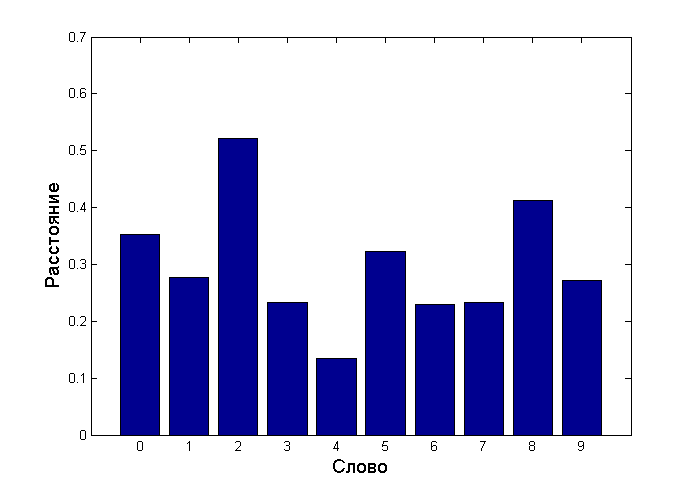
\includegraphics[width=\textwidth]{../clear_4.png}			
			\caption{Значения меры отличий для слова <<четыре>> без влияния шумов}
			\label{clear_4}
		\end{subfigure}
		\begin{subfigure}{0.32\textwidth}	
			\centering
			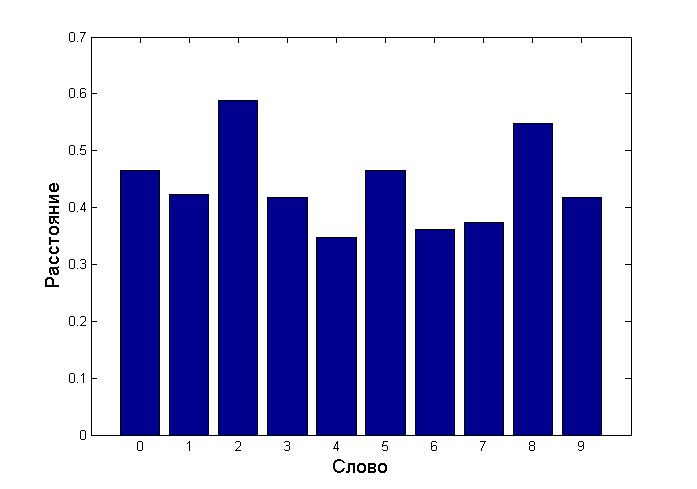
\includegraphics[width=\textwidth]{../60db_4.png}			
			\caption{Значения меры отличий для слова <<четыре>> (отношение сигнал-шум 60 дБ)}
			\label{60db_4}
		\end{subfigure}
		\begin{subfigure}{0.32\textwidth}	
			\centering
			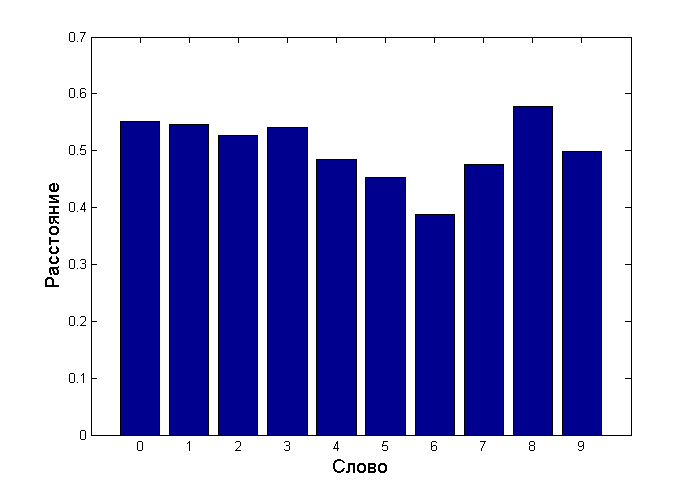
\includegraphics[width=\textwidth]{../40db_4.png}			
			\caption{Значения меры отличий для слова <<четыре>> (отношение сигнал-шум 40 дБ)}
			\label{40db_4}
		\end{subfigure}
		\caption{}
	\end{figure}
\end{frame}

\begin{frame}[plain]
	\frametitle{Алгоритм динамического трансформирования времени}
	Был проведен экспериментальный анализ зависимости точности распознавания от значения отношения сигнал-шум. Для этого вся база из 100 записанных слов сравнивалась с имеющимися эталонами, при этом в каждой итерации из 100 сравнений к анализируемым речевым сигналам добавлялся аддитивный гауссовский белый шум различной мощности.
\end{frame}

\begin{frame}[plain]
	\frametitle{Алгоритм динамического трансформирования времени}
	\begin{figure}[H]	
		\centering
		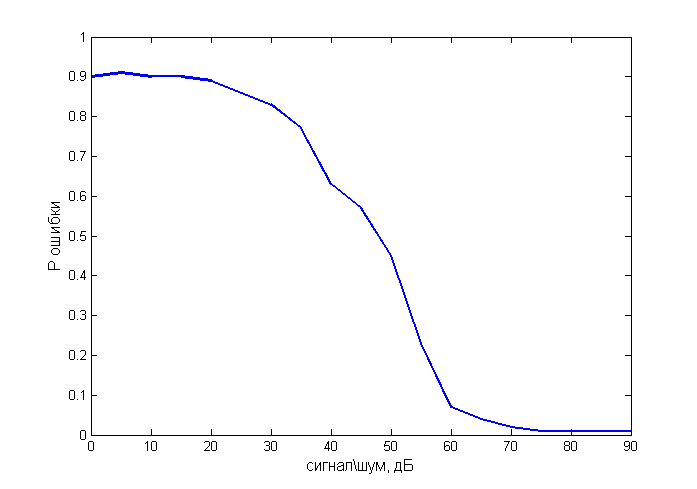
\includegraphics[width=.7\textwidth]{../snr-err.png}			
		\caption{\centering{Зависимость вероятности ошибки распознавания от отношения сигнал-шум}}
		\label{snr-err}
	\end{figure}
\end{frame}

\section{Заключение}
\begin{frame}[squeeze,plain]
	\frametitle{Заключение}
	В ходе выполнения данной работы были решены все поставленные задачи. Изучены существующие подходы к решению проблемы распознавания устной речи, выбран, реализован и исследован один из применяемых алгоритмов.

	Из существующих алгоритмов распознавания устной речи для подробного анализа выбран один --- алгоритм динамического трансформирования времени (DTW), основанный на принципах динамического программирования. Выбор данного алгоритма объясняется возможностью его практической реализации в рамках выпускной квалификационной работы, а также его непосредственной применимостью к задаче распознавания речевых команд в системах с небольшим словарем. Другие известные алгоритмы,  использующие, например, скрытые модели Маркова или нейронные сети, обычно, являются частью систем, реализация которых требует существенных затрат.
	
\end{frame}

\end{document}